\section{Структура сообщества на литорали губы Дальне-Зеленецкой (Восточный Мурман Баренцева моря)} 
\label{app:DZ_soobshestvo_dynamic}
%%%%%%%%%%%%%%%%%%%%%%%%%%%%%%%%%%%%%

	\begin{figure}[hp]
	
	\begin{minipage}[b]{.46\linewidth}
	\begin{center}
	{\footnotesize \textit{Fabricia sabella}}
		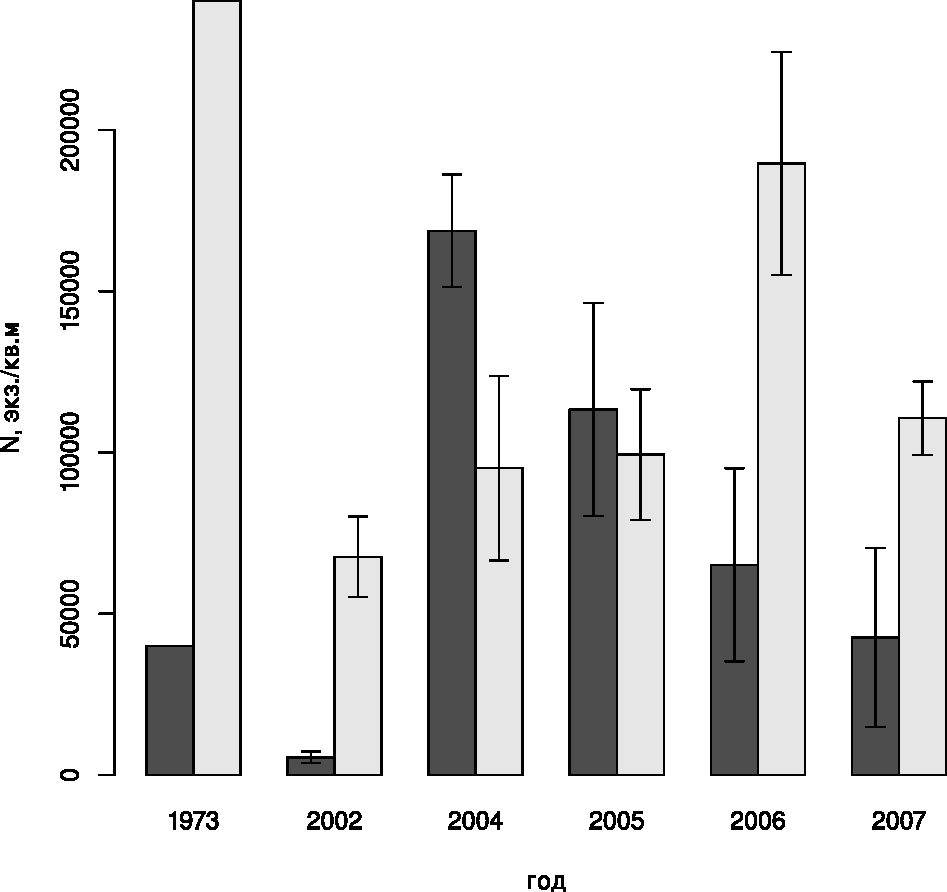
\includegraphics[width=55mm]{../after_Deryuginskie/2_disser/Fabricia_N_dynamic1.pdf}
	\end{center}
	\end{minipage}
	%
	\hfil %Это пружинка отодвигающая рисунки друг от друга
	%
	\begin{minipage}[b]{.46\linewidth}
	\begin{center}
	{\footnotesize \textit{Pygospio elegans}}
		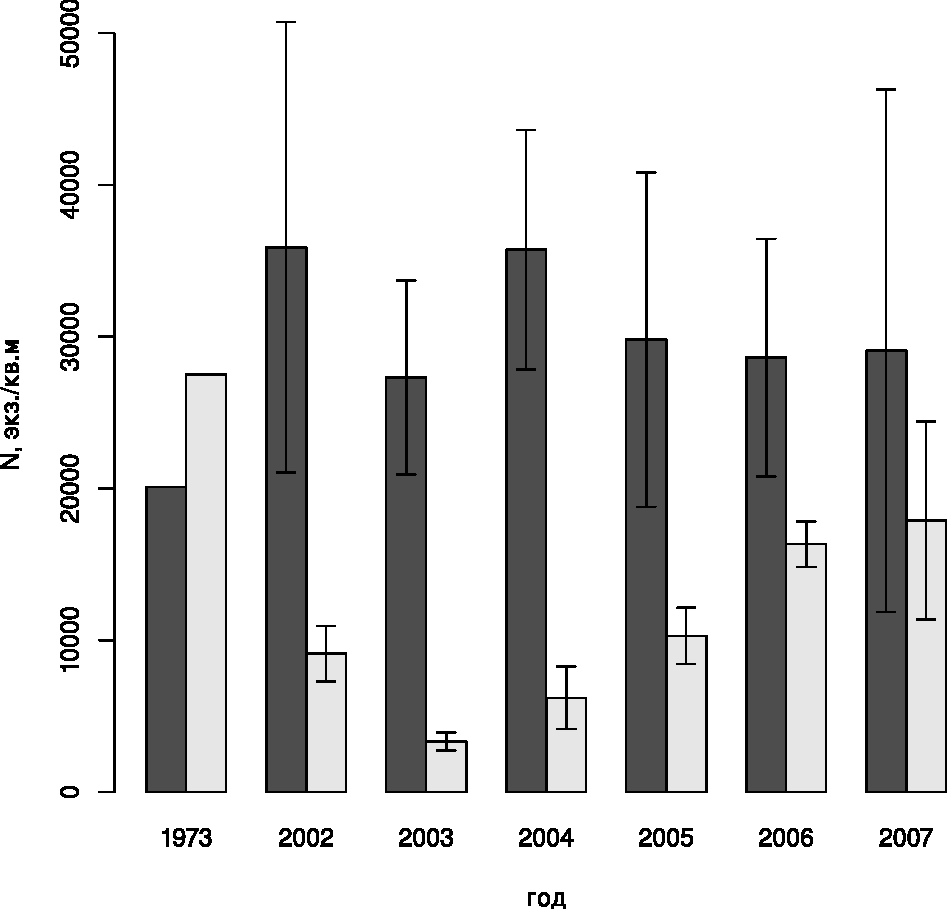
\includegraphics[width=55mm]{../after_Deryuginskie/2_disser/Pygospio_N_dynamic1.pdf}
	\end{center}
	\end{minipage}
	%\smallskip
	\begin{minipage}[b]{.46\linewidth}
	\begin{center}
	{\footnotesize \textit{Arenicola marina}}
	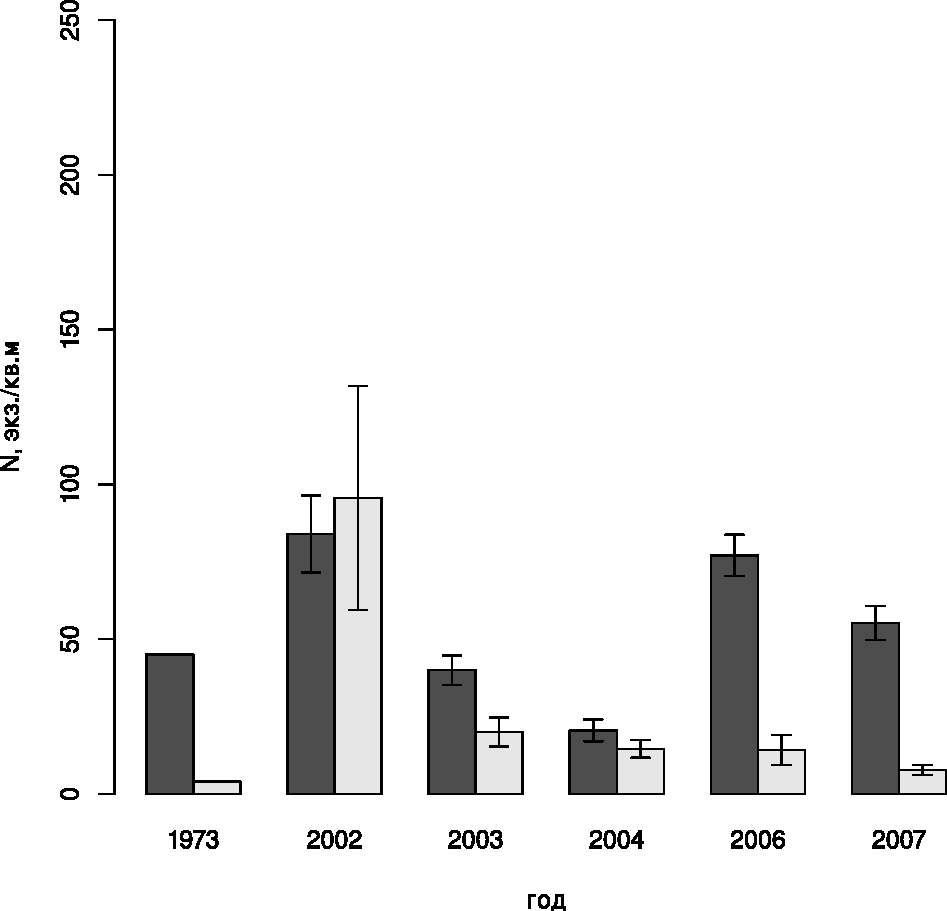
\includegraphics[width=55mm]{../after_Deryuginskie/2_disser/Arenicola_N_dynamic1.pdf}
	\end{center}
	\end{minipage}
	%	
	\hfil %Это пружинка отодвигающая рисунки друг от друга
	%
	\begin{minipage}[b]{.46\linewidth}
	\begin{center}	
	{\footnotesize \textit{Capitella capitata}}
	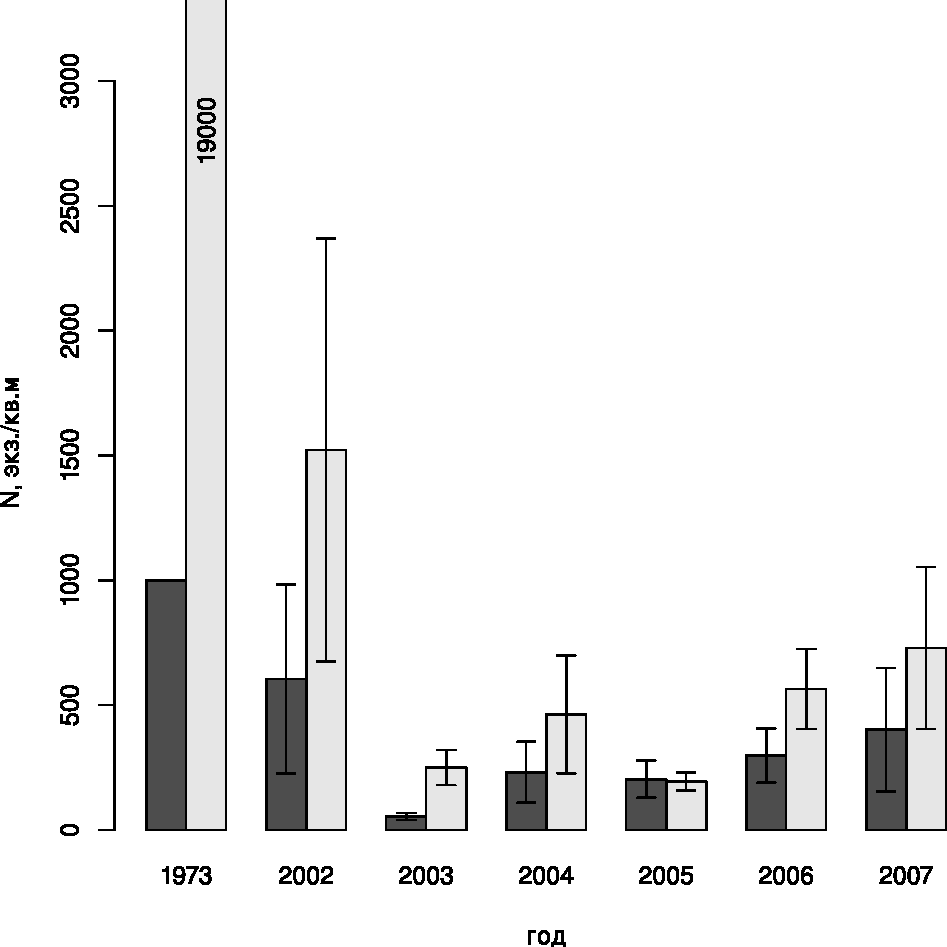
\includegraphics[width=55mm]{../after_Deryuginskie/2_disser/Capitella_N_dynamic1.pdf}
	\end{center}
	\end{minipage}
	%\smallskip
	\begin{minipage}[b]{.46\linewidth}
	\begin{center}
	{\footnotesize Oligochaeta}\\
	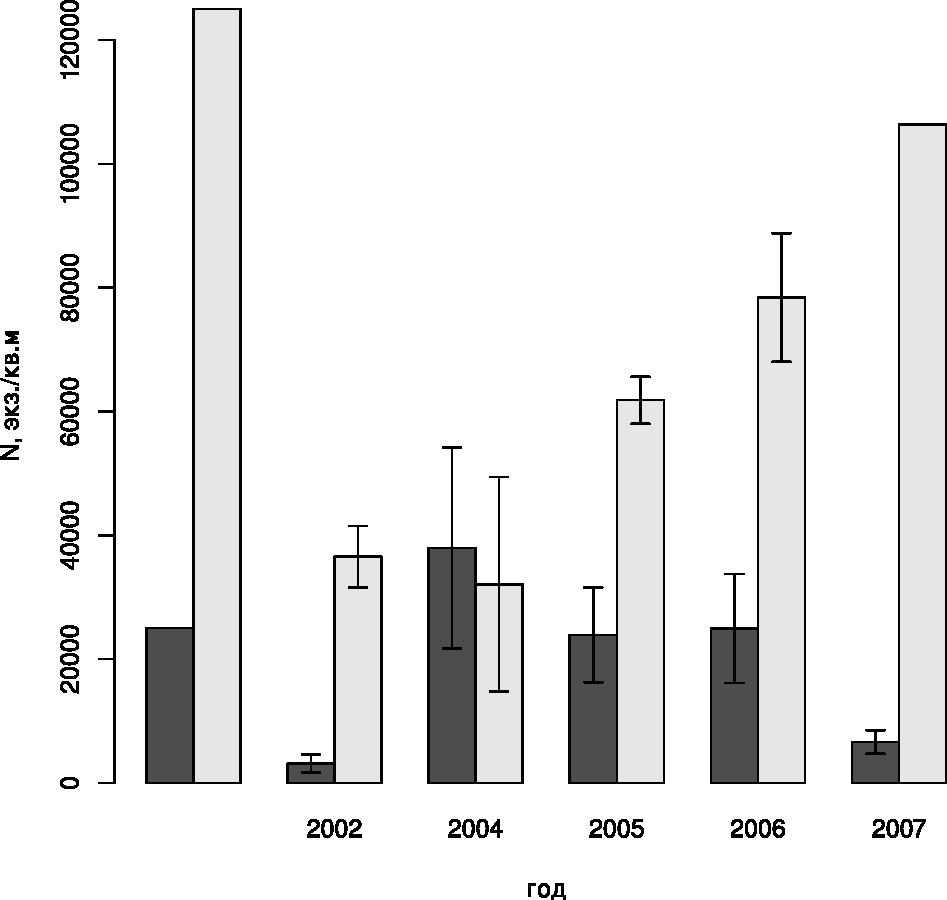
\includegraphics[width=55mm]{../after_Deryuginskie/2_disser/Oligochaeta_N_dynamic1.pdf}
	\end{center}
	\end{minipage}
	%
	\hfil %Это пружинка отодвигающая рисунки друг от друга
	%
	\begin{minipage}[b]{.46\linewidth}
%	\begin{center}
%	{\footnotesize Порчниха, СГЛ}
%	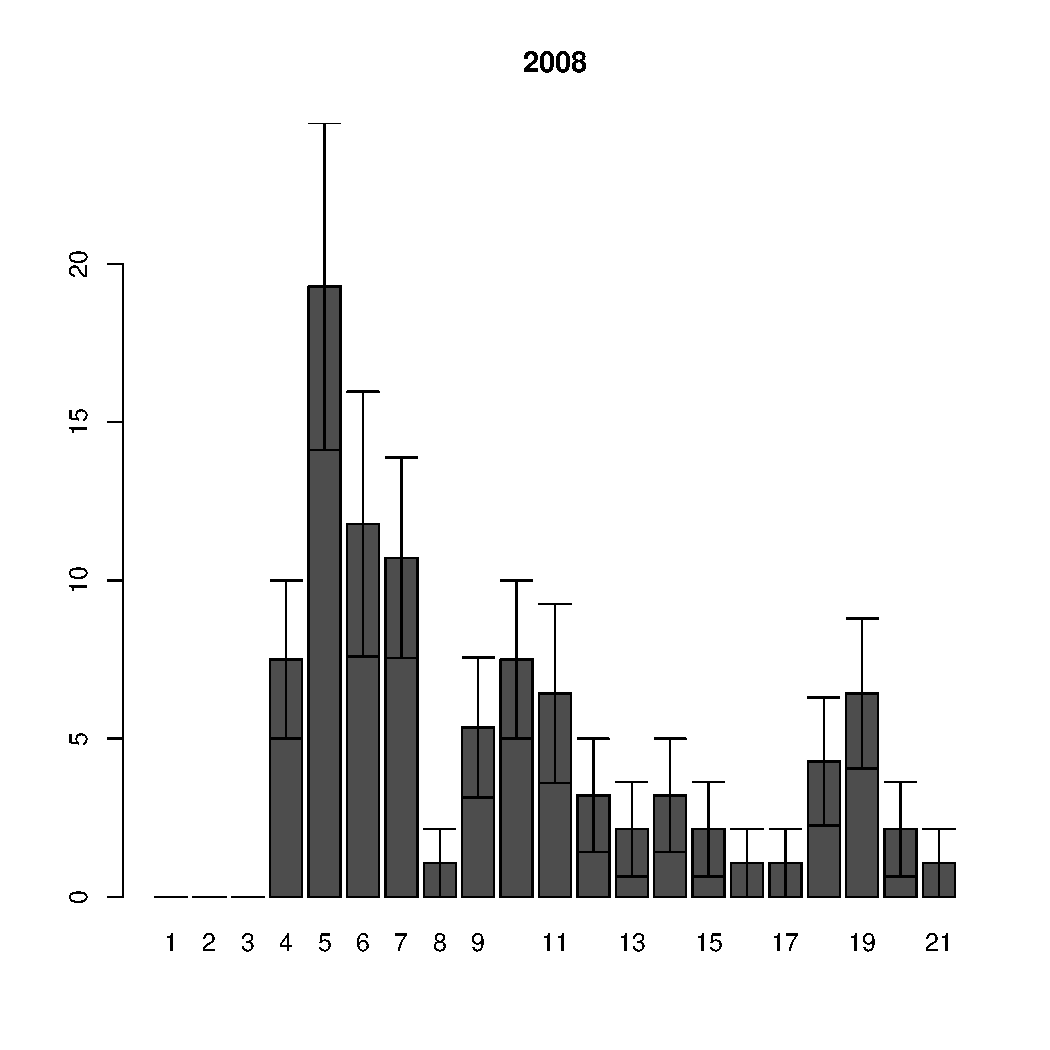
\includegraphics[width=55mm]{../Barenc_Sea/Porchnikha/sizestr2007.pdf}
%	\end{center}
	\end{minipage}
	%\smallskip
\caption{Динамика обилия массовых видов на литорали Дальнего пляжа губы Дальне-Зеленецкой}
\label{ris:DZ_N_dynamic_dominants}

{\footnotesize Примечание: N~--- плотность поселения, экз./м$^2$: темные столбцы~--- в сообществе пескожилов, светлые~--- в сообществе трубкостроителей.}
\end{figure}
